% Options for packages loaded elsewhere
\PassOptionsToPackage{unicode}{hyperref}
\PassOptionsToPackage{hyphens}{url}
%
\documentclass[
]{book}
\usepackage{amsmath,amssymb}
\usepackage{lmodern}
\usepackage{iftex}
\ifPDFTeX
  \usepackage[T1]{fontenc}
  \usepackage[utf8]{inputenc}
  \usepackage{textcomp} % provide euro and other symbols
\else % if luatex or xetex
  \usepackage{unicode-math}
  \defaultfontfeatures{Scale=MatchLowercase}
  \defaultfontfeatures[\rmfamily]{Ligatures=TeX,Scale=1}
\fi
% Use upquote if available, for straight quotes in verbatim environments
\IfFileExists{upquote.sty}{\usepackage{upquote}}{}
\IfFileExists{microtype.sty}{% use microtype if available
  \usepackage[]{microtype}
  \UseMicrotypeSet[protrusion]{basicmath} % disable protrusion for tt fonts
}{}
\makeatletter
\@ifundefined{KOMAClassName}{% if non-KOMA class
  \IfFileExists{parskip.sty}{%
    \usepackage{parskip}
  }{% else
    \setlength{\parindent}{0pt}
    \setlength{\parskip}{6pt plus 2pt minus 1pt}}
}{% if KOMA class
  \KOMAoptions{parskip=half}}
\makeatother
\usepackage{xcolor}
\usepackage{color}
\usepackage{fancyvrb}
\newcommand{\VerbBar}{|}
\newcommand{\VERB}{\Verb[commandchars=\\\{\}]}
\DefineVerbatimEnvironment{Highlighting}{Verbatim}{commandchars=\\\{\}}
% Add ',fontsize=\small' for more characters per line
\usepackage{framed}
\definecolor{shadecolor}{RGB}{248,248,248}
\newenvironment{Shaded}{\begin{snugshade}}{\end{snugshade}}
\newcommand{\AlertTok}[1]{\textcolor[rgb]{0.94,0.16,0.16}{#1}}
\newcommand{\AnnotationTok}[1]{\textcolor[rgb]{0.56,0.35,0.01}{\textbf{\textit{#1}}}}
\newcommand{\AttributeTok}[1]{\textcolor[rgb]{0.77,0.63,0.00}{#1}}
\newcommand{\BaseNTok}[1]{\textcolor[rgb]{0.00,0.00,0.81}{#1}}
\newcommand{\BuiltInTok}[1]{#1}
\newcommand{\CharTok}[1]{\textcolor[rgb]{0.31,0.60,0.02}{#1}}
\newcommand{\CommentTok}[1]{\textcolor[rgb]{0.56,0.35,0.01}{\textit{#1}}}
\newcommand{\CommentVarTok}[1]{\textcolor[rgb]{0.56,0.35,0.01}{\textbf{\textit{#1}}}}
\newcommand{\ConstantTok}[1]{\textcolor[rgb]{0.00,0.00,0.00}{#1}}
\newcommand{\ControlFlowTok}[1]{\textcolor[rgb]{0.13,0.29,0.53}{\textbf{#1}}}
\newcommand{\DataTypeTok}[1]{\textcolor[rgb]{0.13,0.29,0.53}{#1}}
\newcommand{\DecValTok}[1]{\textcolor[rgb]{0.00,0.00,0.81}{#1}}
\newcommand{\DocumentationTok}[1]{\textcolor[rgb]{0.56,0.35,0.01}{\textbf{\textit{#1}}}}
\newcommand{\ErrorTok}[1]{\textcolor[rgb]{0.64,0.00,0.00}{\textbf{#1}}}
\newcommand{\ExtensionTok}[1]{#1}
\newcommand{\FloatTok}[1]{\textcolor[rgb]{0.00,0.00,0.81}{#1}}
\newcommand{\FunctionTok}[1]{\textcolor[rgb]{0.00,0.00,0.00}{#1}}
\newcommand{\ImportTok}[1]{#1}
\newcommand{\InformationTok}[1]{\textcolor[rgb]{0.56,0.35,0.01}{\textbf{\textit{#1}}}}
\newcommand{\KeywordTok}[1]{\textcolor[rgb]{0.13,0.29,0.53}{\textbf{#1}}}
\newcommand{\NormalTok}[1]{#1}
\newcommand{\OperatorTok}[1]{\textcolor[rgb]{0.81,0.36,0.00}{\textbf{#1}}}
\newcommand{\OtherTok}[1]{\textcolor[rgb]{0.56,0.35,0.01}{#1}}
\newcommand{\PreprocessorTok}[1]{\textcolor[rgb]{0.56,0.35,0.01}{\textit{#1}}}
\newcommand{\RegionMarkerTok}[1]{#1}
\newcommand{\SpecialCharTok}[1]{\textcolor[rgb]{0.00,0.00,0.00}{#1}}
\newcommand{\SpecialStringTok}[1]{\textcolor[rgb]{0.31,0.60,0.02}{#1}}
\newcommand{\StringTok}[1]{\textcolor[rgb]{0.31,0.60,0.02}{#1}}
\newcommand{\VariableTok}[1]{\textcolor[rgb]{0.00,0.00,0.00}{#1}}
\newcommand{\VerbatimStringTok}[1]{\textcolor[rgb]{0.31,0.60,0.02}{#1}}
\newcommand{\WarningTok}[1]{\textcolor[rgb]{0.56,0.35,0.01}{\textbf{\textit{#1}}}}
\usepackage{longtable,booktabs,array}
\usepackage{calc} % for calculating minipage widths
% Correct order of tables after \paragraph or \subparagraph
\usepackage{etoolbox}
\makeatletter
\patchcmd\longtable{\par}{\if@noskipsec\mbox{}\fi\par}{}{}
\makeatother
% Allow footnotes in longtable head/foot
\IfFileExists{footnotehyper.sty}{\usepackage{footnotehyper}}{\usepackage{footnote}}
\makesavenoteenv{longtable}
\usepackage{graphicx}
\makeatletter
\def\maxwidth{\ifdim\Gin@nat@width>\linewidth\linewidth\else\Gin@nat@width\fi}
\def\maxheight{\ifdim\Gin@nat@height>\textheight\textheight\else\Gin@nat@height\fi}
\makeatother
% Scale images if necessary, so that they will not overflow the page
% margins by default, and it is still possible to overwrite the defaults
% using explicit options in \includegraphics[width, height, ...]{}
\setkeys{Gin}{width=\maxwidth,height=\maxheight,keepaspectratio}
% Set default figure placement to htbp
\makeatletter
\def\fps@figure{htbp}
\makeatother
\setlength{\emergencystretch}{3em} % prevent overfull lines
\providecommand{\tightlist}{%
  \setlength{\itemsep}{0pt}\setlength{\parskip}{0pt}}
\setcounter{secnumdepth}{5}
\usepackage{booktabs}
\ifLuaTeX
  \usepackage{selnolig}  % disable illegal ligatures
\fi
\usepackage[]{natbib}
\bibliographystyle{apalike}
\IfFileExists{bookmark.sty}{\usepackage{bookmark}}{\usepackage{hyperref}}
\IfFileExists{xurl.sty}{\usepackage{xurl}}{} % add URL line breaks if available
\urlstyle{same} % disable monospaced font for URLs
\hypersetup{
  pdftitle={Advanced Measurement Theory Course Notebook},
  pdfauthor={William M. Murrah},
  hidelinks,
  pdfcreator={LaTeX via pandoc}}

\title{Advanced Measurement Theory Course Notebook}
\author{William M. Murrah}
<<<<<<< HEAD:docs/AdvancedMeasurementTheoryNotebook.tex
\date{2022-12-10}
=======
\date{2022-12-11}
>>>>>>> Quartobook:_book/_main.tex

\begin{document}
\maketitle

{
\setcounter{tocdepth}{1}
\tableofcontents
}
\hypertarget{introduction-to-the-course}{%
\chapter*{Introduction to the Course}\label{introduction-to-the-course}}
\addcontentsline{toc}{chapter}{Introduction to the Course}

Welcome!
This is a notebook for ERMA 8350 Advanced Measurement Theory.
<<<<<<< HEAD:docs/AdvancedMeasurementTheoryNotebook.tex
The class will be using the textbook \emph{Handbook of Educational Measurement and Psychometrics Using R}, which will be the primary source for the course .
I will use this notebook to make available additional information to help you learn the material.
=======
The class will be using the textbook \emph{Handbook of Educational Measurement and Psychometrics Using R} \citep{Desjardins2018Handbookeducationalmeasurement}, which will be the primary source for learning to use R for the methods covered in this course.
I will use this notebook to make available additional readings to help you learn the theory behind these methods and to provide published examples of their use.
>>>>>>> Quartobook:_book/_main.tex
It may include some examples from the textbook, with some elaborations, additional readings, and some more details about implementing the methods in R.
These web-based notes will make it easy for you to use code, by allowing you to copy and paste code found within.
Some of you will have experience with R and others not.
So I will try to also point you to additional resources that may be helpful.
For example, in this preface I will provide links to resources to help you setup R and RStudio.
RStudio is a platform to make using R more productive.
<<<<<<< HEAD:docs/AdvancedMeasurementTheoryNotebook.tex
I will use it extensively in this course \citep{Desjardins2018Handbookeducationalmeasurement}.
=======
I will use it extensively in this course.
>>>>>>> Quartobook:_book/_main.tex

There are at least two way you can access the software needed for this course.
You can use the virtual labs on campus.
I know at least the education virtual labs have R and RStudio installed.
IF you go this route you can watch the following video.
Note you will need Duo setup for this to work.

\href{https://nv.instructuremedia.com/fetch/QkFoYkIxc0hhUVNIRGFrSE1Hd3JCeWhUREdFPS0tZjk4ODFlYWEyZWFiNWQwYWYyZDk0YTZjMjljZTJlMjBkNmIwMzE5Yw.mp4}{Using Vlab to acces R/RStudio}

A better option if you have a laptop, you can install both programs on your computer.
They are both absolutely free and available on all major operating systems, so you will not have to worry about transferring information across computers, limited connection speeds, or other hassles inherent with the VLab route.

The following links take you to videos instructing you how to install them.

\href{https://auburn.hosted.panopto.com/Panopto/Pages/Viewer.aspx?id=5dacd1fe-b888-407b-a89f-ac150135ace8}{Installing R and RStudio}

\href{https://auburn.hosted.panopto.com/Panopto/Pages/Viewer.aspx?id=aed0e2a9-004f-453f-80c7-abbe010a063b}{Organizing Projects in RStudio}

\hypertarget{resources-for-learning-r}{%
\section*{Resources for Learning R}\label{resources-for-learning-r}}
\addcontentsline{toc}{section}{Resources for Learning R}

While such experience is certainly helpful, I do not assume you have prior knowledge of using R.
I will demonstrate the use of R and provide (particularly in this notebook) the R code needed to use the methods we will learn.
However, even if you have prior experience with R, you should plan to spend time learning to program in R.
Some people find this intimidating initially, but most of you will grow to find R programming rewarding, and even fun by the end of the course.
But, there will be frustration for sure.

Here are some good places to start learning R:

\href{https://cran.r-project.org/}{CRAN}

\hypertarget{r-packages}{%
\section*{R Packages}\label{r-packages}}
\addcontentsline{toc}{section}{R Packages}

R is, among other paradigms, a functional programming language, which means is heavily utilizes functions.
R's functions are stored in packages.
While base R has a long list of very useful functions, to fully realize the power of R you will have to use additional packages.
So, learning how to \textbf{install} packages (downloading from the web to your computer) and \textbf{loading} packages (making the package's functions accessible to your current R session) are important skills to master.

\hypertarget{how-to-use-these-notes}{%
\section*{How To Use These Notes}\label{how-to-use-these-notes}}
\addcontentsline{toc}{section}{How To Use These Notes}

Before going further, it may be helpful to watch the following video about how to use the code in this notebook with Rstudio:

\href{https://auburn.hosted.panopto.com/Panopto/Pages/Viewer.aspx?id=13acb849-902a-45c7-bc4e-ad870153fcae}{How to Use RStudio with this Notebook}

\hypertarget{generalizability-theory}{%
\chapter{Generalizability Theory}\label{generalizability-theory}}

We describe our methods in this chapter.

\hypertarget{generalizability-theory-1}{%
\chapter{Generalizability Theory}\label{generalizability-theory-1}}

We describe our methods in this chapter.

\hypertarget{factor-analysis}{%
\chapter{Factor Analysis}\label{factor-analysis}}

\hypertarget{correlation-coefficient}{%
\section{Correlation Coefficient}\label{correlation-coefficient}}

\emph{Pearson product-moment correlation}:

\[
r_{xy} = \frac{\Sigma_{n=1}^n (x_k - \bar{x})(y_i - \bar{y})}{\sqrt{\Sigma_{n=1}^n(x_i - \bar{x})^2} \sqrt{\Sigma_{n=1}^n(y_i - \bar{y})^2}} = \frac{s_{xy}}{s_x s_y}.
\]

The equation looks very daunting, until you see that it is just the covariance of \(x\) and \(y\) divided by the product of their standard deviations.

\begin{Shaded}
\begin{Highlighting}[]
\FunctionTok{library}\NormalTok{(}\StringTok{"MPsychoR"}\NormalTok{)}
\FunctionTok{data}\NormalTok{(}\StringTok{"YouthDep"}\NormalTok{)}
\NormalTok{item1 }\OtherTok{\textless{}{-}}\NormalTok{ YouthDep[, }\DecValTok{1}\NormalTok{]}
\FunctionTok{levels}\NormalTok{(item1) }\OtherTok{\textless{}{-}} \FunctionTok{c}\NormalTok{(}\StringTok{"0"}\NormalTok{, }\StringTok{"1"}\NormalTok{, }\StringTok{"1"}\NormalTok{)}
\NormalTok{item2 }\OtherTok{\textless{}{-}}\NormalTok{ YouthDep[, }\DecValTok{14}\NormalTok{]}
\FunctionTok{levels}\NormalTok{(item2) }\OtherTok{\textless{}{-}} \FunctionTok{c}\NormalTok{(}\StringTok{"0"}\NormalTok{, }\StringTok{"1"}\NormalTok{, }\StringTok{"1"}\NormalTok{)}
\FunctionTok{table}\NormalTok{(item1, item2)}
\end{Highlighting}
\end{Shaded}

\begin{verbatim}
     item2
item1    0    1
    0 1353  656
    1  115  166
\end{verbatim}

\begin{Shaded}
\begin{Highlighting}[]
\DocumentationTok{\#\# {-}{-}{-}{-}{-}{-} correlation coefficients}
\FunctionTok{library}\NormalTok{(}\StringTok{"psych"}\NormalTok{)}
\NormalTok{tetcor }\OtherTok{\textless{}{-}} \FunctionTok{tetrachoric}\NormalTok{(}\FunctionTok{cbind}\NormalTok{(item1, item2))}
\end{Highlighting}
\end{Shaded}

\begin{Shaded}
\begin{Highlighting}[]
\NormalTok{tetcor}
\end{Highlighting}
\end{Shaded}

\begin{verbatim}
Call: tetrachoric(x = cbind(item1, item2))
tetrachoric correlation 
      item1 item2
item1 1.00       
item2 0.35  1.00 

 with tau of 
item1 item2 
 1.16  0.36 
\end{verbatim}

\begin{Shaded}
\begin{Highlighting}[]
\NormalTok{item1 }\OtherTok{\textless{}{-}}\NormalTok{ YouthDep[, }\DecValTok{1}\NormalTok{]}
\NormalTok{item2 }\OtherTok{\textless{}{-}}\NormalTok{ YouthDep[, }\DecValTok{14}\NormalTok{]}
\NormalTok{polcor }\OtherTok{\textless{}{-}} \FunctionTok{polychoric}\NormalTok{(}\FunctionTok{cbind}\NormalTok{(item1, item2))}
\NormalTok{polcor}
\end{Highlighting}
\end{Shaded}

\begin{verbatim}
Call: polychoric(x = cbind(item1, item2))
Polychoric correlations 
      item1 item2
item1 1.00       
item2 0.33  1.00 

 with tau of 
         1   2
item1 1.16 2.3
item2 0.36 1.2
\end{verbatim}

\begin{Shaded}
\begin{Highlighting}[]
\FunctionTok{draw.tetra}\NormalTok{(}\AttributeTok{r =}\NormalTok{ .}\DecValTok{35}\NormalTok{, }\AttributeTok{t1 =} \FloatTok{1.16}\NormalTok{, }\AttributeTok{t2 =}\NormalTok{ .}\DecValTok{36}\NormalTok{)}
\end{Highlighting}
\end{Shaded}

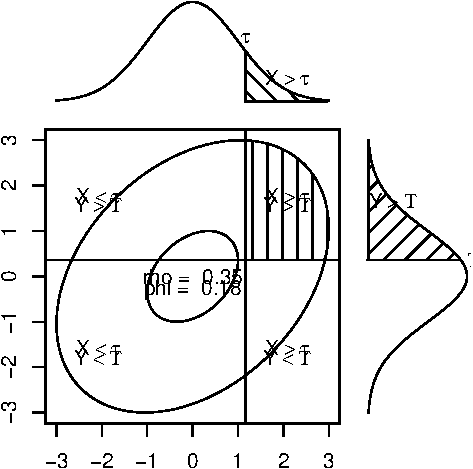
\includegraphics{_main_files/figure-latex/unnamed-chunk-3-1.pdf}

\begin{Shaded}
\begin{Highlighting}[]
\NormalTok{DepItems }\OtherTok{\textless{}{-}}\NormalTok{ YouthDep[,}\DecValTok{1}\SpecialCharTok{:}\DecValTok{26}\NormalTok{] }
\NormalTok{Depnum }\OtherTok{\textless{}{-}} \FunctionTok{data.matrix}\NormalTok{(DepItems) }\SpecialCharTok{{-}} \DecValTok{1}  \DocumentationTok{\#\# convert to numeric   }
\NormalTok{Rdep }\OtherTok{\textless{}{-}} \FunctionTok{polychoric}\NormalTok{(Depnum)}
\end{Highlighting}
\end{Shaded}

\hypertarget{think-about-these-situations}{%
\section{Think about these situations}\label{think-about-these-situations}}

What do you do when you have a large number of variables you are considering as predictors of a dependent variable?

\begin{itemize}
\tightlist
\item
  Often, subsets of these variables are measuring the same, or very similar things.
\item
  We might like to reduce the variables to a smaller number of predictors.
\end{itemize}

What if you are developing a measurement scale and have a large number of items you think measure the same construct

\begin{itemize}
\tightlist
\item
  You might want to see how strongly the items are related to the construct.
\end{itemize}

\hypertarget{solutions}{%
\section{Solutions}\label{solutions}}

\begin{enumerate}
\def\labelenumi{\arabic{enumi}.}
\item
  Principal Components Analysis

  \begin{itemize}
  \tightlist
  \item
    transforming the original variables into a new set of linear combinations (pricipal components).
  \end{itemize}
\item
  Factor Analysis

  \begin{itemize}
  \tightlist
  \item
    setting up a mathematical model to estimate the number or factors
  \end{itemize}
\end{enumerate}

\hypertarget{principal-components-analysis}{%
\section{Principal Components Analysis}\label{principal-components-analysis}}

\begin{itemize}
\tightlist
\item
  Concerned with explaining variance-covariance structure of a set of variables.
\item
  PCA attempts to explain as much of the total variance among the observed variables as possible with a smaller number of components.
\item
  Because the variables are standardized prior to analysis, the total amount of variance available is the number of variables.
\item
  The goal is \textbf{data reduction} for subsequent analysis.
\item
  Variables \emph{cause} components.
\item
  Components are not representative of any underlying theory.
\end{itemize}

\hypertarget{factor-analysis-1}{%
\section{Factor Analysis}\label{factor-analysis-1}}

\begin{itemize}
\tightlist
\item
  The goal is understanding underlying constructs.
\item
  Uses a modified correlation matrix (reduced matrix)
\item
  factors \emph{cause} the variables.
\item
  Factors represent theoretical constructs.
\item
  Focuses on the common variance of the variables, and purges the unique variance.
\end{itemize}

\hypertarget{components}{%
\section{Components}\label{components}}

The principal components partition the total variance (the sum of the variances of the original variables) by finding the linear combination of the variables that account for the maximum amount of variance:

\[
PC1 = a_{11}x_1 + a_{12}x_2 ... a_{1p}x_p, 
\]
This is repeated as many time as there are variables.

\hypertarget{pc-extraction}{%
\section{PC Extraction}\label{pc-extraction}}

draw pretty pictures on the board

\hypertarget{eigenvalues}{%
\section{Eigenvalues}\label{eigenvalues}}

Eigenvalues represent the variance in the variables explained by the success components.

\hypertarget{determining-the-number-of-factors}{%
\section{Determining the Number of Factors}\label{determining-the-number-of-factors}}

\begin{enumerate}
\def\labelenumi{\arabic{enumi}.}
\tightlist
\item
  Kaiser criterion: Retain only factors with eigenvalues \textgreater{} 1. (generally accurate)
\item
  Scree plot: plot eigenvalues and drop factors after leveling off.
\item
  Parallel analysis: compare observed eigenvalues to parallel set of data from randomly generated data. Retain factors in original if eigenvalue is greater than random eigenvalue.
\item
  Factor meaningfulness is also very important to consider.
\end{enumerate}

\hypertarget{example-data}{%
\section{Example data}\label{example-data}}

\begin{Shaded}
\begin{Highlighting}[]
\NormalTok{lower }\OtherTok{\textless{}{-}} \StringTok{"}
\StringTok{1.00}
\StringTok{0.70 1.00}
\StringTok{0.65 0.66 1.00}
\StringTok{0.62 0.63 0.60 1.00}
\StringTok{"}
\NormalTok{cormat }\OtherTok{\textless{}{-}} \FunctionTok{getCov}\NormalTok{(lower, }\AttributeTok{names =} \FunctionTok{c}\NormalTok{(}\StringTok{"d1"}\NormalTok{, }\StringTok{"d2"}\NormalTok{, }\StringTok{"d3"}\NormalTok{, }\StringTok{"d4"}\NormalTok{))}

\NormalTok{cormat}
\end{Highlighting}
\end{Shaded}

\begin{verbatim}
     d1   d2   d3   d4
d1 1.00 0.70 0.65 0.62
d2 0.70 1.00 0.66 0.63
d3 0.65 0.66 1.00 0.60
d4 0.62 0.63 0.60 1.00
\end{verbatim}

\hypertarget{kaiser}{%
\section{Kaiser}\label{kaiser}}

Retain factors with eigenvalues greater than 1

\begin{Shaded}
\begin{Highlighting}[]
\FunctionTok{eigen}\NormalTok{(cormat)}\SpecialCharTok{$}\NormalTok{values}
\end{Highlighting}
\end{Shaded}

\begin{verbatim}
[1] 2.9311792 0.4103921 0.3592372 0.2991916
\end{verbatim}

\hypertarget{scree-plot}{%
\section{Scree Plot}\label{scree-plot}}

\begin{Shaded}
\begin{Highlighting}[]
\FunctionTok{scree}\NormalTok{(cormat, }\AttributeTok{factors =} \ConstantTok{FALSE}\NormalTok{)}
\end{Highlighting}
\end{Shaded}

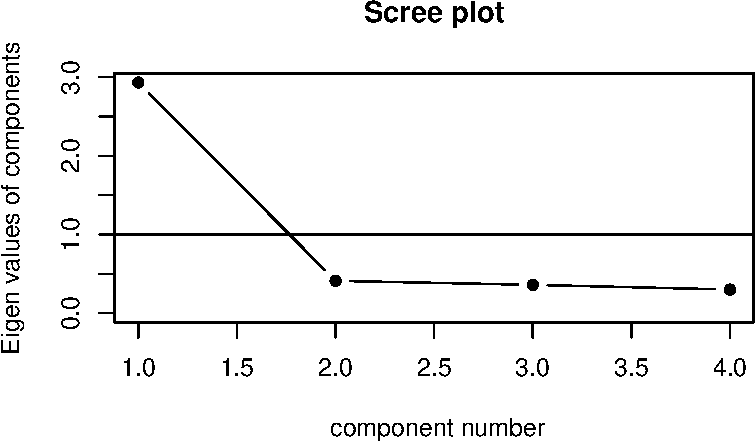
\includegraphics{_main_files/figure-latex/unnamed-chunk-6-1.pdf}

\hypertarget{horns-parallel-analysis}{%
\section{Horn's Parallel Analysis}\label{horns-parallel-analysis}}

\begin{Shaded}
\begin{Highlighting}[]
\FunctionTok{fa.parallel}\NormalTok{(cormat, }\AttributeTok{fa =} \StringTok{"pc"}\NormalTok{)}
\end{Highlighting}
\end{Shaded}

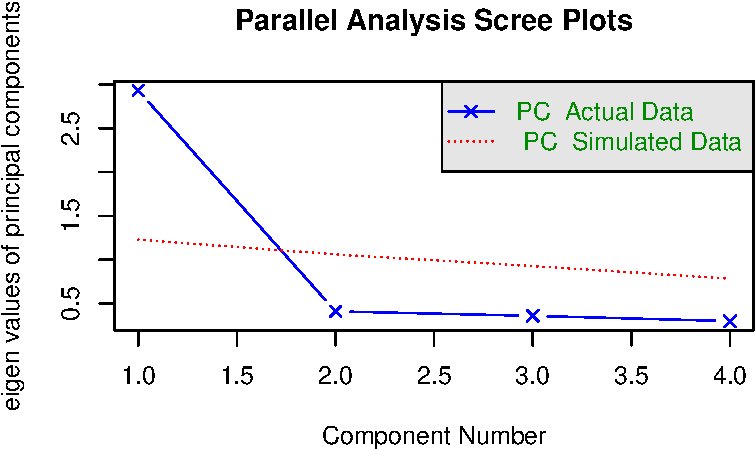
\includegraphics{_main_files/figure-latex/unnamed-chunk-7-1.pdf}

\begin{verbatim}
Parallel analysis suggests that the number of factors =  NA  and the number of components =  1 
\end{verbatim}

\hypertarget{another-example}{%
\section{Another example}\label{another-example}}

\begin{Shaded}
\begin{Highlighting}[]
\FunctionTok{fa.parallel}\NormalTok{(Harman74.cor}\SpecialCharTok{$}\NormalTok{cov, }\AttributeTok{fa =} \StringTok{"pc"}\NormalTok{)}
\end{Highlighting}
\end{Shaded}

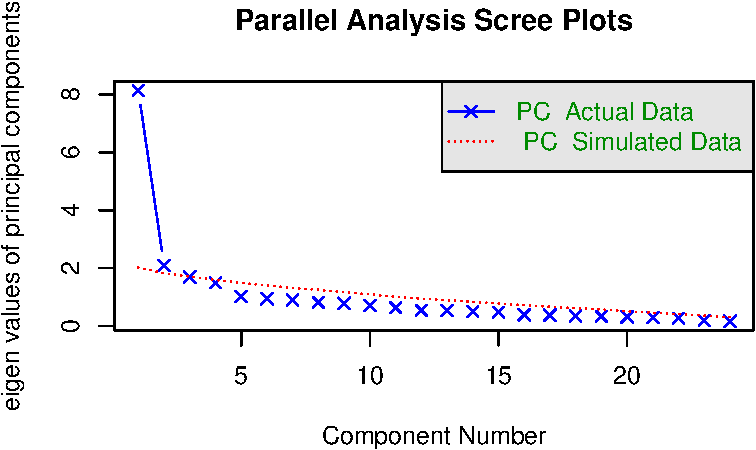
\includegraphics{_main_files/figure-latex/unnamed-chunk-8-1.pdf}

\begin{verbatim}
Parallel analysis suggests that the number of factors =  NA  and the number of components =  2 
\end{verbatim}

\hypertarget{rotation}{%
\section{Rotation}\label{rotation}}

\begin{itemize}
\tightlist
\item
  Principal components are derived to maximize the variance accounted for (data reduction).
\item
  Rotation is done to make the factors more interpretable (i.e.~meaningful).
\item
  Two major classes of rotation:

  \begin{itemize}
  \tightlist
  \item
    Orthogonal - new factors are still uncorrelated, as were the initial factors.
  \item
    Oblique - new factors are allowed to be correlated.
  \end{itemize}
\end{itemize}

Essentially reallocates the loadings. The first factor may not be the one accounting for the most variance.

\hypertarget{orthogonal-rotation}{%
\section{Orthogonal Rotation}\label{orthogonal-rotation}}

\begin{enumerate}
\def\labelenumi{\arabic{enumi}.}
\item
  \textbf{Quartimax} - idea is to clean up the \emph{variables}. Rotation done so each variable loads mainly on one factor. Problematic if there is a general factor on which most or all variables load on (think IQ).
\item
  \textbf{Varimax} - to clean up \emph{factors}. So each factor has high correlation with a smaller number of variables, low correlation with the other variables. Generally makes interpretation easier.
\end{enumerate}

\hypertarget{oblique-rotation}{%
\section{Oblique Rotation}\label{oblique-rotation}}

\begin{itemize}
\tightlist
\item
  Often correlated factors are more reasonable.
\item
  Therefore, oblique rotation is often preferred.
\item
  But interpretation is more complicated.
\end{itemize}

\hypertarget{factor-matrices}{%
\section{Factor Matrices}\label{factor-matrices}}

\begin{enumerate}
\def\labelenumi{\arabic{enumi}.}
\tightlist
\item
  Factor pattern matrix:

  \begin{itemize}
  \tightlist
  \item
    includes \emph{pattern coefficients} analogous to standardized partial regression coefficients.
  \item
    Indicated the unique importance of a factor to a variable, holding other factors constant.
  \end{itemize}
\item
  Factor structure matrix:

  \begin{itemize}
  \tightlist
  \item
    includes \emph{structure coefficients} which are simple correlations of the variables with the factors.
  \end{itemize}
\end{enumerate}

\hypertarget{which-matrix-should-we-interpret}{%
\section{Which matrix should we interpret?}\label{which-matrix-should-we-interpret}}

\begin{itemize}
\item
  When orthogonal rotation is used interpret \emph{structural coefficients} (but they are the same as pattern coefficients).
\item
  When oblique rotation is used pattern coefficients are preferred because they account for the correlation between the factors and they are parameters of the correlated factor model (which we will discuss next class).
\end{itemize}

\hypertarget{which-variables-should-be-used-to-interpret-each-factor}{%
\section{Which variables should be used to interpret each factor?}\label{which-variables-should-be-used-to-interpret-each-factor}}

\begin{itemize}
\tightlist
\item
  The idea is to use only those variables that have a strong association with the factor.
\item
  Typical thresholds are \textbar.30\textbar{} or \textbar.40\textbar.
\item
  Content knowledge is critical.
\end{itemize}

\hypertarget{examples}{%
\section{Examples}\label{examples}}

Let's look at some examples

\hypertarget{steps-in-factor-analysis}{%
\section{Steps in Factor Analysis}\label{steps-in-factor-analysis}}

\begin{enumerate}
\def\labelenumi{\arabic{enumi}.}
\tightlist
\item
  Choose extraction method

  \begin{itemize}
  \tightlist
  \item
    So far we've focused on PCA
  \end{itemize}
\item
  Determine the number of components/factors

  \begin{itemize}
  \tightlist
  \item
    Kaiser method: eigenvalues \textgreater{} 1
  \item
    Scree plot: All components before leveling off
  \item
    Horn's parallel analysis: components/factors greater than simulated values from random numbers
  \end{itemize}
\item
  Rotate Factors

  \begin{itemize}
  \tightlist
  \item
    Orthogonal
  \item
    Oblique
  \end{itemize}
\item
  Interpret Components/Factors
\end{enumerate}

\hypertarget{tom-swifts-electric-factor-analysis-factory}{%
\section{Tom Swift's Electric Factor Analysis Factory}\label{tom-swifts-electric-factor-analysis-factory}}

``Little Jiffy'' method of factor analysis

\begin{enumerate}
\def\labelenumi{\arabic{enumi}.}
\tightlist
\item
  Extraction method : PCA
\item
  Number of factors: eigenvalues \textgreater{} 1
\item
  Rotation: orthogonal(varimax)
\item
  Interpretation
\end{enumerate}

\hypertarget{metal-boxes}{%
\section{Metal Boxes}\label{metal-boxes}}

\begin{table}

\caption{\label{tab:unnamed-chunk-10}Functional Definitions of Tom Swift's Original 11 Variables}
\centering
\begin{tabular}[t]{l|l}
\hline
Dimension & Derivation\\
\hline
Thickness & x\\
\hline
Width & y\\
\hline
Length & z\\
\hline
Volume & xyz\\
\hline
Density & d\\
\hline
Weight & xyzd\\
\hline
Surface area & 2(xy + xz + yz)\\
\hline
Cross-section & yz\\
\hline
Edge length & 4(x + y + z)\\
\hline
Diagonal length & (x\textasciicircum{}2)\\
\hline
Cost/lb & c\\
\hline
\end{tabular}
\end{table}

\begin{verbatim}
'data.frame':   63 obs. of  11 variables:
 $ thick   : num  1.362 2.385 3.101 0.934 0.845 ...
 $ width   : num  1.71 2.83 4.32 3.2 3.84 ...
 $ length  : num  2.93 5.01 5.99 4.15 4.09 ...
 $ volume  : num  6.02 30.2 72.01 11.78 16.1 ...
 $ density : int  10 7 16 22 11 16 11 21 6 13 ...
 $ weight  : num  60 210 1152 264 176 ...
 $ surface : num  22 62.1 108.2 38 48 ...
 $ crosssec: num  5.87 15.06 23.53 12.02 16.13 ...
 $ edge    : num  23.9 39.9 51.5 31.9 36.1 ...
 $ diagonal: num  196 1444 3721 676 1089 ...
 $ cost    : num  4.48 2.37 9.77 22.21 15.86 ...
\end{verbatim}

\begin{table}[]
\begin{tabular}{lllll}
 Dimension &  Derivation  &  \\
 \hline \\
 Thickness &  $x$  \\
 Width & $y$ \\
 Length & $z$ \\
 Volume & $xyz$ \\
 Density & $d$ \\
 Weight & $xyzd$ \\
 Total surface area & $2(xy + xz +_ yz)$ \\
 Cross-sectional area & $yz$ \\
 Total edge length & $4(x +  y + z)$ \\
 Internal diagonal length & $(x^2 + y^2 + z^2)^2$ \\
 Cost per pound & $c$
\end{tabular}
\end{table}

\hypertarget{correlations}{%
\section{Correlations}\label{correlations}}

\tiny
\begin{table}

\caption{\label{tab:unnamed-chunk-12}Correlations between dimensions}
\centering
\begin{tabular}[t]{l|r|r|r|r|r|r|r|r|r|r|r}
\hline
  & thick & width & length & volume & density & weight & surface & crosssec & edge & diagonal & cost\\
\hline
thick & 1.00 & 0.49 & 0.24 & 0.84 & -0.13 & 0.59 & 0.74 & 0.46 & 0.61 & 0.51 & -0.02\\
\hline
width & 0.49 & 1.00 & 0.61 & 0.77 & -0.15 & 0.55 & 0.87 & 0.92 & 0.88 & 0.78 & 0.03\\
\hline
length & 0.24 & 0.61 & 1.00 & 0.58 & -0.02 & 0.45 & 0.72 & 0.83 & 0.84 & 0.86 & -0.02\\
\hline
volume & 0.84 & 0.77 & 0.58 & 1.00 & -0.22 & 0.65 & 0.97 & 0.81 & 0.87 & 0.85 & -0.11\\
\hline
density & -0.13 & -0.15 & -0.02 & -0.22 & 1.00 & 0.44 & -0.20 & -0.15 & -0.15 & -0.18 & 0.62\\
\hline
weight & 0.59 & 0.55 & 0.45 & 0.65 & 0.44 & 1.00 & 0.65 & 0.56 & 0.61 & 0.57 & 0.24\\
\hline
surface & 0.74 & 0.87 & 0.72 & 0.97 & -0.20 & 0.65 & 1.00 & 0.92 & 0.97 & 0.91 & -0.07\\
\hline
crosssec & 0.46 & 0.92 & 0.83 & 0.81 & -0.15 & 0.56 & 0.92 & 1.00 & 0.96 & 0.93 & -0.03\\
\hline
edge & 0.61 & 0.88 & 0.84 & 0.87 & -0.15 & 0.61 & 0.97 & 0.96 & 1.00 & 0.92 & -0.04\\
\hline
diagonal & 0.51 & 0.78 & 0.86 & 0.85 & -0.18 & 0.57 & 0.91 & 0.93 & 0.92 & 1.00 & -0.12\\
\hline
cost & -0.02 & 0.03 & -0.02 & -0.11 & 0.62 & 0.24 & -0.07 & -0.03 & -0.04 & -0.12 & 1.00\\
\hline
\end{tabular}
\end{table}

\hypertarget{eigenvalues-1}{%
\section{Eigenvalues \textgreater{} 1}\label{eigenvalues-1}}

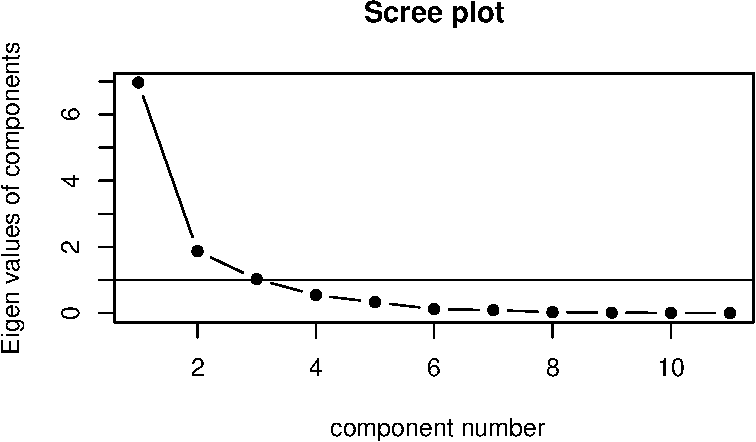
\includegraphics{_main_files/figure-latex/unnamed-chunk-13-1.pdf}

\hypertarget{orthogonal-rotation-1}{%
\section{Orthogonal Rotation}\label{orthogonal-rotation-1}}

\footnotesize

\begin{verbatim}

Loadings:
         RC1    RC3    RC2    RC5    RC4   
thick            0.968                     
width                          0.734       
length    0.986                            
volume           0.754                     
density                 0.864              
weight                                     
surface   0.703                            
crosssec  0.829                            
edge      0.819                            
diagonal  0.875                            
cost                                  0.955

                 RC1   RC3   RC2   RC5   RC4
SS loadings    4.425 2.662 1.318 1.225 1.106
Proportion Var 0.402 0.242 0.120 0.111 0.101
Cumulative Var 0.402 0.644 0.764 0.876 0.976
\end{verbatim}

\hypertarget{orthogonal-rotation-with-loadings-.70}{%
\section{Orthogonal Rotation with Loadings \textgreater{} .70}\label{orthogonal-rotation-with-loadings-.70}}

\footnotesize

\begin{verbatim}

Loadings:
         RC1    RC3    RC2   
thick            0.947       
width     0.801              
length    0.936              
volume           0.744       
density                 0.930
weight                       
surface   0.792              
crosssec  0.942              
edge      0.892              
diagonal  0.905              
cost                    0.841

                 RC1   RC3   RC2
SS loadings    5.298 2.699 1.868
Proportion Var 0.482 0.245 0.170
Cumulative Var 0.482 0.727 0.897
\end{verbatim}

\hypertarget{r-code-for-chapter-2}{%
\section{R Code for Chapter 2}\label{r-code-for-chapter-2}}

\begin{Shaded}
\begin{Highlighting}[]
\DocumentationTok{\#\# {-}{-}{-}{-}{-}{-}{-}{-}{-}{-}{-}{-}{-}{-}{-}{-}{-}{-}{-}{-}{-}{-}{-} Chapter 2: Factor Analysis {-}{-}{-}{-}{-}{-}{-}{-}{-}{-}{-}{-}{-}{-}{-}{-}{-}{-}}
\FunctionTok{library}\NormalTok{(}\StringTok{"MPsychoR"}\NormalTok{)}
\FunctionTok{data}\NormalTok{(}\StringTok{"YouthDep"}\NormalTok{)}
\NormalTok{item1 }\OtherTok{\textless{}{-}}\NormalTok{ YouthDep[, }\DecValTok{1}\NormalTok{]}
\FunctionTok{levels}\NormalTok{(item1) }\OtherTok{\textless{}{-}} \FunctionTok{c}\NormalTok{(}\StringTok{"0"}\NormalTok{, }\StringTok{"1"}\NormalTok{, }\StringTok{"1"}\NormalTok{)}
\NormalTok{item2 }\OtherTok{\textless{}{-}}\NormalTok{ YouthDep[, }\DecValTok{14}\NormalTok{]}
\FunctionTok{levels}\NormalTok{(item2) }\OtherTok{\textless{}{-}} \FunctionTok{c}\NormalTok{(}\StringTok{"0"}\NormalTok{, }\StringTok{"1"}\NormalTok{, }\StringTok{"1"}\NormalTok{)}
\FunctionTok{table}\NormalTok{(item1, item2)}

\DocumentationTok{\#\# {-}{-}{-}{-}{-}{-} correlation coefficients}
\FunctionTok{library}\NormalTok{(}\StringTok{"psych"}\NormalTok{)}
\NormalTok{tetcor }\OtherTok{\textless{}{-}} \FunctionTok{tetrachoric}\NormalTok{(}\FunctionTok{cbind}\NormalTok{(item1, item2))}
\NormalTok{tetcor}
\NormalTok{item1 }\OtherTok{\textless{}{-}}\NormalTok{ YouthDep[, }\DecValTok{1}\NormalTok{]}
\NormalTok{item2 }\OtherTok{\textless{}{-}}\NormalTok{ YouthDep[, }\DecValTok{14}\NormalTok{]}
\NormalTok{polcor }\OtherTok{\textless{}{-}} \FunctionTok{polychoric}\NormalTok{(}\FunctionTok{cbind}\NormalTok{(item1, item2))}
\NormalTok{polcor}

\NormalTok{DepItems }\OtherTok{\textless{}{-}}\NormalTok{ YouthDep[,}\DecValTok{1}\SpecialCharTok{:}\DecValTok{26}\NormalTok{] }
\NormalTok{Depnum }\OtherTok{\textless{}{-}} \FunctionTok{data.matrix}\NormalTok{(DepItems) }\SpecialCharTok{{-}} \DecValTok{1}  \DocumentationTok{\#\# convert to numeric   }
\NormalTok{Rdep }\OtherTok{\textless{}{-}} \FunctionTok{polychoric}\NormalTok{(Depnum)}

\FunctionTok{data}\NormalTok{(}\StringTok{"Rmotivation"}\NormalTok{)}
\NormalTok{vind }\OtherTok{\textless{}{-}} \FunctionTok{grep}\NormalTok{(}\StringTok{"ext|int"}\NormalTok{, }\FunctionTok{colnames}\NormalTok{(Rmotivation)) }
\NormalTok{Rmotivation1 }\OtherTok{\textless{}{-}}\NormalTok{ Rmotivation[, vind]}
\NormalTok{Rmot1 }\OtherTok{\textless{}{-}} \FunctionTok{tetrachoric}\NormalTok{(Rmotivation1, }\AttributeTok{smooth =} \ConstantTok{FALSE}\NormalTok{)}
\FunctionTok{tail}\NormalTok{(}\FunctionTok{round}\NormalTok{(}\FunctionTok{eigen}\NormalTok{(Rmot1}\SpecialCharTok{$}\NormalTok{rho)}\SpecialCharTok{$}\NormalTok{values, }\DecValTok{3}\NormalTok{))}
\NormalTok{Rmot }\OtherTok{\textless{}{-}} \FunctionTok{tetrachoric}\NormalTok{(Rmotivation1)}
\FunctionTok{tail}\NormalTok{(}\FunctionTok{round}\NormalTok{(}\FunctionTok{eigen}\NormalTok{(Rmot}\SpecialCharTok{$}\NormalTok{rho)}\SpecialCharTok{$}\NormalTok{values, }\DecValTok{3}\NormalTok{))}

\DocumentationTok{\#\# {-}{-}{-}{-}{-} exploratory factor analysis }
\NormalTok{motFA }\OtherTok{\textless{}{-}} \FunctionTok{fa}\NormalTok{(Rmot}\SpecialCharTok{$}\NormalTok{rho, }\AttributeTok{nfactors =} \DecValTok{2}\NormalTok{, }\AttributeTok{rotate =} \StringTok{"none"}\NormalTok{, }\AttributeTok{fm =} \StringTok{"ml"}\NormalTok{)}
\FunctionTok{print}\NormalTok{(motFA}\SpecialCharTok{$}\NormalTok{loadings, }\AttributeTok{cutoff =} \FloatTok{0.2}\NormalTok{)}
\FunctionTok{round}\NormalTok{(motFA}\SpecialCharTok{$}\NormalTok{communality, }\DecValTok{2}\NormalTok{)}

\NormalTok{motFA2 }\OtherTok{\textless{}{-}} \FunctionTok{fa}\NormalTok{(Rmot}\SpecialCharTok{$}\NormalTok{rho, }\AttributeTok{nfactors =} \DecValTok{2}\NormalTok{, }\AttributeTok{rotate =} \StringTok{"varimax"}\NormalTok{, }\AttributeTok{fm =} \StringTok{"ml"}\NormalTok{)}
\FunctionTok{plot}\NormalTok{(motFA}\SpecialCharTok{$}\NormalTok{loadings, }\AttributeTok{asp =} \DecValTok{1}\NormalTok{, }\AttributeTok{xlim =} \FunctionTok{c}\NormalTok{(}\SpecialCharTok{{-}}\FloatTok{0.2}\NormalTok{, }\FloatTok{0.9}\NormalTok{), }\AttributeTok{ylim =} \FunctionTok{c}\NormalTok{(}\SpecialCharTok{{-}}\FloatTok{0.5}\NormalTok{, }\FloatTok{0.9}\NormalTok{), }\AttributeTok{type =} \StringTok{"n"}\NormalTok{, }\AttributeTok{xlab =} \StringTok{"Factor 1"}\NormalTok{, }\AttributeTok{ylab =} \StringTok{"Factor 2"}\NormalTok{, }\AttributeTok{main =} \StringTok{"Loadings Plot"}\NormalTok{)}
\FunctionTok{text}\NormalTok{(motFA}\SpecialCharTok{$}\NormalTok{loadings, }\AttributeTok{labels =} \FunctionTok{rownames}\NormalTok{(motFA}\SpecialCharTok{$}\NormalTok{loadings), }\AttributeTok{cex =} \FloatTok{0.8}\NormalTok{, }\AttributeTok{col =} \StringTok{"gray"}\NormalTok{)}
\FunctionTok{abline}\NormalTok{(}\AttributeTok{h =} \DecValTok{0}\NormalTok{, }\AttributeTok{v =} \DecValTok{0}\NormalTok{, }\AttributeTok{col =} \StringTok{"lightgray"}\NormalTok{, }\AttributeTok{lty =} \DecValTok{2}\NormalTok{)}
\FunctionTok{text}\NormalTok{(motFA2}\SpecialCharTok{$}\NormalTok{loadings, }\AttributeTok{labels =} \FunctionTok{rownames}\NormalTok{(motFA2}\SpecialCharTok{$}\NormalTok{loadings), }\AttributeTok{col =} \DecValTok{1}\NormalTok{, }\AttributeTok{cex =} \FloatTok{0.8}\NormalTok{)}
\FunctionTok{legend}\NormalTok{(}\StringTok{"bottomleft"}\NormalTok{, }\AttributeTok{legend =} \FunctionTok{c}\NormalTok{(}\StringTok{"rotated"}\NormalTok{, }\StringTok{"unrotated"}\NormalTok{), }\AttributeTok{col =} \FunctionTok{c}\NormalTok{(}\StringTok{"black"}\NormalTok{, }\StringTok{"gray"}\NormalTok{), }\AttributeTok{pch =} \DecValTok{19}\NormalTok{)}

\NormalTok{Rmot2 }\OtherTok{\textless{}{-}} \FunctionTok{tetrachoric}\NormalTok{(Rmotivation[,}\DecValTok{1}\SpecialCharTok{:}\DecValTok{36}\NormalTok{])}
\NormalTok{motFA3 }\OtherTok{\textless{}{-}} \FunctionTok{fa}\NormalTok{(Rmot2}\SpecialCharTok{$}\NormalTok{rho, }\AttributeTok{nfactors =} \DecValTok{3}\NormalTok{, }\AttributeTok{rotate =} \StringTok{"oblimin"}\NormalTok{, }\AttributeTok{fm =} \StringTok{"ml"}\NormalTok{)}
\NormalTok{motFA3}\SpecialCharTok{$}\NormalTok{loadings}
\FunctionTok{round}\NormalTok{(motFA3}\SpecialCharTok{$}\NormalTok{Phi, }\DecValTok{3}\NormalTok{)}

\NormalTok{motFA2 }\OtherTok{\textless{}{-}} \FunctionTok{fa}\NormalTok{(Rmotivation1, }\AttributeTok{nfactors =} \DecValTok{2}\NormalTok{, }\AttributeTok{rotate =} \StringTok{"varimax"}\NormalTok{, }\AttributeTok{cor =} \StringTok{"tet"}\NormalTok{, }\AttributeTok{fm =} \StringTok{"ml"}\NormalTok{, }\AttributeTok{scores =} \StringTok{"regression"}\NormalTok{,}
             \AttributeTok{missing =} \ConstantTok{TRUE}\NormalTok{, }\AttributeTok{impute =} \StringTok{"median"}\NormalTok{)}
\FunctionTok{dim}\NormalTok{(motFA2}\SpecialCharTok{$}\NormalTok{scores)}

\NormalTok{Rdep }\OtherTok{\textless{}{-}} \FunctionTok{polychoric}\NormalTok{(Depnum)}\SpecialCharTok{$}\NormalTok{rho}
\NormalTok{evals }\OtherTok{\textless{}{-}} \FunctionTok{eigen}\NormalTok{(Rdep)}\SpecialCharTok{$}\NormalTok{values}
\FunctionTok{scree}\NormalTok{(Rdep, }\AttributeTok{factors =} \ConstantTok{FALSE}\NormalTok{)}
\NormalTok{(evals}\SpecialCharTok{/}\FunctionTok{sum}\NormalTok{(evals)}\SpecialCharTok{*}\DecValTok{100}\NormalTok{)[}\DecValTok{1}\SpecialCharTok{:}\DecValTok{2}\NormalTok{]}

\FunctionTok{set.seed}\NormalTok{(}\DecValTok{123}\NormalTok{)}
\NormalTok{resPA }\OtherTok{\textless{}{-}} \FunctionTok{fa.parallel}\NormalTok{(Depnum, }\AttributeTok{fa =} \StringTok{"pc"}\NormalTok{, }\AttributeTok{cor =} \StringTok{"poly"}\NormalTok{, }\AttributeTok{fm =} \StringTok{"ml"}\NormalTok{)  }
\NormalTok{resvss }\OtherTok{\textless{}{-}} \FunctionTok{vss}\NormalTok{(Rdep, }\AttributeTok{fm =} \StringTok{"ml"}\NormalTok{, }\AttributeTok{n.obs =} \FunctionTok{nrow}\NormalTok{(Depnum), }\AttributeTok{plot =} \ConstantTok{FALSE}\NormalTok{)}
\NormalTok{resvss}

\NormalTok{fadep }\OtherTok{\textless{}{-}} \FunctionTok{fa}\NormalTok{(Depnum, }\DecValTok{1}\NormalTok{, }\AttributeTok{cor =} \StringTok{"poly"}\NormalTok{, }\AttributeTok{fm =} \StringTok{"ml"}\NormalTok{)}
\FunctionTok{summary}\NormalTok{(fadep)}

\NormalTok{resnf }\OtherTok{\textless{}{-}} \FunctionTok{nfactors}\NormalTok{(Depnum, }\AttributeTok{n =} \DecValTok{8}\NormalTok{, }\AttributeTok{fm =} \StringTok{"ml"}\NormalTok{, }\AttributeTok{cor =} \StringTok{"poly"}\NormalTok{)}
\NormalTok{resnf}

\DocumentationTok{\#\# {-}{-}{-}{-}{-} Bayesian exploratory factor analysis}
\FunctionTok{library}\NormalTok{(}\StringTok{"MPsychoR"}\NormalTok{)}
\FunctionTok{library}\NormalTok{(}\StringTok{"corrplot"}\NormalTok{)}
\FunctionTok{library}\NormalTok{(}\StringTok{"BayesFM"}\NormalTok{)}
\FunctionTok{data}\NormalTok{(}\StringTok{"Privacy"}\NormalTok{)}
\NormalTok{Privstd }\OtherTok{\textless{}{-}} \FunctionTok{scale}\NormalTok{(Privacy)}
\FunctionTok{corrplot}\NormalTok{(}\FunctionTok{cor}\NormalTok{(Privstd))}

\NormalTok{Nid }\OtherTok{\textless{}{-}} \DecValTok{2}              \DocumentationTok{\#\# minimum number of variables per factor}
\NormalTok{pmax }\OtherTok{\textless{}{-}} \FunctionTok{trunc}\NormalTok{(}\FunctionTok{ncol}\NormalTok{(Privstd)}\SpecialCharTok{/}\NormalTok{Nid)   }\DocumentationTok{\#\# maximum number of factors}
\NormalTok{pmax}

\FunctionTok{set.seed}\NormalTok{(}\DecValTok{123}\NormalTok{)}
\NormalTok{Rsim }\OtherTok{\textless{}{-}} \FunctionTok{simul.R.prior}\NormalTok{(pmax, }\AttributeTok{nu0 =}\NormalTok{ pmax }\SpecialCharTok{+} \FunctionTok{c}\NormalTok{(}\DecValTok{1}\NormalTok{, }\DecValTok{2}\NormalTok{, }\DecValTok{5}\NormalTok{, }\DecValTok{7}\NormalTok{, }\DecValTok{10}\NormalTok{))}
\FunctionTok{plot}\NormalTok{(Rsim)}

\NormalTok{Ksim }\OtherTok{\textless{}{-}} \FunctionTok{simul.nfac.prior}\NormalTok{(}\AttributeTok{nvar =} \FunctionTok{ncol}\NormalTok{(Privstd), }\AttributeTok{Nid =}\NormalTok{ Nid, }\AttributeTok{Kmax =}\NormalTok{ pmax, }\AttributeTok{kappa =} \FunctionTok{c}\NormalTok{(.}\DecValTok{1}\NormalTok{, .}\DecValTok{2}\NormalTok{, .}\DecValTok{5}\NormalTok{, }\DecValTok{1}\NormalTok{))}
\FunctionTok{plot}\NormalTok{(Ksim)}

\FunctionTok{set.seed}\NormalTok{(}\DecValTok{222}\NormalTok{)}
\NormalTok{fitbefa }\OtherTok{\textless{}{-}} \FunctionTok{befa}\NormalTok{(Privstd, }\AttributeTok{Nid =} \DecValTok{2}\NormalTok{, }\AttributeTok{Kmax =}\NormalTok{ pmax, }\AttributeTok{nu0 =} \DecValTok{10}\NormalTok{, }\AttributeTok{kappa =} \FloatTok{0.2}\NormalTok{, }\AttributeTok{kappa0 =} \FloatTok{0.1}\NormalTok{, }\AttributeTok{xi0 =} \FloatTok{0.1}\NormalTok{,}
                \AttributeTok{burnin =} \DecValTok{5000}\NormalTok{, }\AttributeTok{iter =} \DecValTok{50000}\NormalTok{)}
\NormalTok{fitbefa }\OtherTok{\textless{}{-}} \FunctionTok{post.column.switch}\NormalTok{(fitbefa)   }\DocumentationTok{\#\# column reordering}
\NormalTok{fitbefa }\OtherTok{\textless{}{-}} \FunctionTok{post.sign.switch}\NormalTok{(fitbefa)     }\DocumentationTok{\#\# sign switching}
\NormalTok{sumbefa }\OtherTok{\textless{}{-}} \FunctionTok{summary}\NormalTok{(fitbefa)}

\DocumentationTok{\#\# {-}{-}{-}{-}{-} confirmatory factor analysis}
\FunctionTok{library}\NormalTok{(}\StringTok{"MPsychoR"}\NormalTok{)}
\FunctionTok{library}\NormalTok{(}\StringTok{"lavaan"}\NormalTok{)}
\FunctionTok{data}\NormalTok{(}\StringTok{"Rmotivation"}\NormalTok{)}
\NormalTok{vind }\OtherTok{\textless{}{-}} \FunctionTok{grep}\NormalTok{(}\StringTok{"ext|int"}\NormalTok{, }\FunctionTok{colnames}\NormalTok{(Rmotivation)) }\DocumentationTok{\#\# ext/int items}
\NormalTok{Rmot }\OtherTok{\textless{}{-}} \FunctionTok{na.omit}\NormalTok{(Rmotivation[, vind])}
\NormalTok{mot\_model }\OtherTok{\textless{}{-}} \StringTok{\textquotesingle{} }
\StringTok{  extrinsic  =\textasciitilde{} ext1 + ext2 + ext3 + ext4 + ext5 + ext6 + }
\StringTok{                ext7 + ext8 + ext9 + ext10 + ext11 + ext12      }
\StringTok{  intrinsic =\textasciitilde{}  int1 + int2 + int3 + int4 + int5\textquotesingle{}}
\NormalTok{fitMot }\OtherTok{\textless{}{-}}\NormalTok{ lavaan}\SpecialCharTok{::}\FunctionTok{cfa}\NormalTok{(mot\_model, }\AttributeTok{data =}\NormalTok{ Rmot, }\AttributeTok{ordered =} \FunctionTok{names}\NormalTok{(Rmot))}

\FunctionTok{library}\NormalTok{(}\StringTok{"semPlot"}\NormalTok{)}
\FunctionTok{semPaths}\NormalTok{(fitMot, }\AttributeTok{what =} \StringTok{"est"}\NormalTok{, }\AttributeTok{edge.label.cex =} \FloatTok{0.7}\NormalTok{, }\AttributeTok{edge.color =} \DecValTok{1}\NormalTok{, }\AttributeTok{esize =} \DecValTok{1}\NormalTok{, }\AttributeTok{sizeMan =} \FloatTok{4.5}\NormalTok{, }\AttributeTok{asize =} \FloatTok{2.5}\NormalTok{,}
         \AttributeTok{intercepts =} \ConstantTok{FALSE}\NormalTok{, }\AttributeTok{rotation =} \DecValTok{4}\NormalTok{, }\AttributeTok{thresholdColor =} \StringTok{"red"}\NormalTok{, }\AttributeTok{mar =} \FunctionTok{c}\NormalTok{(}\DecValTok{1}\NormalTok{, }\DecValTok{5}\NormalTok{, }\FloatTok{1.5}\NormalTok{, }\DecValTok{5}\NormalTok{), }\AttributeTok{fade =} \ConstantTok{FALSE}\NormalTok{, }\AttributeTok{nCharNodes =} \DecValTok{4}\NormalTok{)}

\FunctionTok{inspect}\NormalTok{(fitMot, }\AttributeTok{what =} \StringTok{"est"}\NormalTok{)}\SpecialCharTok{$}\NormalTok{theta}
\FunctionTok{inspect}\NormalTok{(fitMot, }\AttributeTok{what =} \StringTok{"est"}\NormalTok{)}\SpecialCharTok{$}\NormalTok{lambda}
\FunctionTok{inspect}\NormalTok{(fitMot, }\AttributeTok{what =} \StringTok{"std"}\NormalTok{)}\SpecialCharTok{$}\NormalTok{lambda}
\FunctionTok{inspect}\NormalTok{(fitMot, }\AttributeTok{what =} \StringTok{"est"}\NormalTok{)}\SpecialCharTok{$}\NormalTok{psi}
\FunctionTok{inspect}\NormalTok{(fitMot, }\AttributeTok{what =} \StringTok{"std"}\NormalTok{)}\SpecialCharTok{$}\NormalTok{psi}

\FunctionTok{parameterEstimates}\NormalTok{(fitMot, }\AttributeTok{standardized =} \ConstantTok{TRUE}\NormalTok{)}
\FunctionTok{summary}\NormalTok{(fitMot, }\AttributeTok{standardized =} \ConstantTok{TRUE}\NormalTok{, }\AttributeTok{fit.measures =} \ConstantTok{TRUE}\NormalTok{)}
\FunctionTok{parameterEstimates}\NormalTok{(fitMot)[}\DecValTok{5}\NormalTok{,]}

\NormalTok{mot\_model2 }\OtherTok{\textless{}{-}} \StringTok{\textquotesingle{}}
\StringTok{  extrinsic  =\textasciitilde{} ext1 + ext2 + ext3 + ext4 + ext6 + ext7 + }
\StringTok{                ext8 + ext9 + ext10 + ext11 + ext12}
\StringTok{  intrinsic =\textasciitilde{}  int1 + int2 + int3 + int4 + int5\textquotesingle{}}
\NormalTok{fitMot2 }\OtherTok{\textless{}{-}}\NormalTok{ lavaan}\SpecialCharTok{::}\FunctionTok{cfa}\NormalTok{(mot\_model2, }\AttributeTok{data =}\NormalTok{ Rmot, }\AttributeTok{ordered =} \FunctionTok{names}\NormalTok{(Rmot)[}\SpecialCharTok{{-}}\DecValTok{5}\NormalTok{])}
\NormalTok{vind }\OtherTok{\textless{}{-}} \FunctionTok{c}\NormalTok{(}\DecValTok{1}\SpecialCharTok{:}\DecValTok{4}\NormalTok{, }\DecValTok{13}\SpecialCharTok{:}\DecValTok{16}\NormalTok{, }\DecValTok{32}\SpecialCharTok{:}\DecValTok{35}\NormalTok{)}
\NormalTok{Rmot2 }\OtherTok{\textless{}{-}} \FunctionTok{na.omit}\NormalTok{(Rmotivation[, vind])}

\NormalTok{mot\_model3 }\OtherTok{\textless{}{-}} \StringTok{\textquotesingle{}}
\StringTok{  extrinsic  =\textasciitilde{} ext1 + ext2 + ext3 + ext4 }
\StringTok{  hybrid =\textasciitilde{} hyb1 + hyb2 + hyb3 + hyb4              }
\StringTok{  intrinsic =\textasciitilde{}  int1 + int2 + int3 + int4 }
\StringTok{  motivation =\textasciitilde{} extrinsic + hybrid + intrinsic\textquotesingle{}}
\NormalTok{fitMot3 }\OtherTok{\textless{}{-}}\NormalTok{ lavaan}\SpecialCharTok{::}\FunctionTok{cfa}\NormalTok{(mot\_model3, }\AttributeTok{data =}\NormalTok{ Rmot2, }\AttributeTok{ordered =} \FunctionTok{names}\NormalTok{(Rmot2))}

\FunctionTok{semPaths}\NormalTok{(fitMot3, }\AttributeTok{what =} \StringTok{"std"}\NormalTok{, }\AttributeTok{edge.label.cex =} \FloatTok{0.7}\NormalTok{, }\AttributeTok{edge.color =} \DecValTok{1}\NormalTok{, }\AttributeTok{esize =} \DecValTok{1}\NormalTok{, }\AttributeTok{sizeMan =} \DecValTok{5}\NormalTok{, }\AttributeTok{asize =} \FloatTok{2.5}\NormalTok{,}
         \AttributeTok{intercepts =} \ConstantTok{FALSE}\NormalTok{, }\AttributeTok{rotation =} \DecValTok{4}\NormalTok{, }\AttributeTok{thresholdColor =} \StringTok{"red"}\NormalTok{, }\AttributeTok{mar =} \FunctionTok{c}\NormalTok{(}\DecValTok{1}\NormalTok{, }\DecValTok{5}\NormalTok{, }\FloatTok{1.5}\NormalTok{, }\DecValTok{5}\NormalTok{), }\AttributeTok{fade =} \ConstantTok{FALSE}\NormalTok{, }\AttributeTok{nCharNodes =} \DecValTok{4}\NormalTok{)}

\FunctionTok{summary}\NormalTok{(fitMot3, }\AttributeTok{standardized =} \ConstantTok{TRUE}\NormalTok{, }\AttributeTok{fit.measures =} \ConstantTok{TRUE}\NormalTok{)}

\NormalTok{vind }\OtherTok{\textless{}{-}} \FunctionTok{c}\NormalTok{(}\DecValTok{1}\SpecialCharTok{:}\DecValTok{4}\NormalTok{, }\DecValTok{13}\SpecialCharTok{:}\DecValTok{16}\NormalTok{, }\DecValTok{32}\SpecialCharTok{:}\DecValTok{35}\NormalTok{, }\DecValTok{39}\SpecialCharTok{:}\DecValTok{41}\NormalTok{)}
\NormalTok{Rmot3 }\OtherTok{\textless{}{-}} \FunctionTok{na.omit}\NormalTok{(Rmotivation[, vind])}
\NormalTok{mot\_model4 }\OtherTok{\textless{}{-}} \StringTok{\textquotesingle{}}
\StringTok{  extrinsic  =\textasciitilde{} ext1 + ext2 + ext3 + ext4 }
\StringTok{  hybrid =\textasciitilde{} hyb1 + hyb2 + hyb3 + hyb4              }
\StringTok{  intrinsic =\textasciitilde{}  int1 + int2 + int3 + int4 }
\StringTok{  motivation =\textasciitilde{} extrinsic + hybrid + intrinsic}
\StringTok{  motivation \textasciitilde{} npkgs + phd\textquotesingle{}}
\NormalTok{fitMot4 }\OtherTok{\textless{}{-}}\NormalTok{ lavaan}\SpecialCharTok{::}\FunctionTok{cfa}\NormalTok{(mot\_model4, }\AttributeTok{data =}\NormalTok{ Rmot3, }\AttributeTok{ordered =} \FunctionTok{names}\NormalTok{(Rmot3[}\DecValTok{1}\SpecialCharTok{:}\DecValTok{12}\NormalTok{]))}

\FunctionTok{semPaths}\NormalTok{(fitMot4, }\AttributeTok{what =} \StringTok{"std"}\NormalTok{, }\AttributeTok{edge.label.cex =} \FloatTok{0.7}\NormalTok{, }\AttributeTok{edge.color =} \DecValTok{1}\NormalTok{, }\AttributeTok{esize =} \DecValTok{1}\NormalTok{, }\AttributeTok{sizeMan =} \DecValTok{5}\NormalTok{, }\AttributeTok{asize =} \FloatTok{2.5}\NormalTok{,}
         \AttributeTok{intercepts =} \ConstantTok{FALSE}\NormalTok{, }\AttributeTok{rotation =} \DecValTok{4}\NormalTok{, }\AttributeTok{thresholdColor =} \StringTok{"red"}\NormalTok{, }\AttributeTok{mar =} \FunctionTok{c}\NormalTok{(}\DecValTok{1}\NormalTok{, }\DecValTok{5}\NormalTok{, }\FloatTok{1.5}\NormalTok{, }\DecValTok{5}\NormalTok{), }\AttributeTok{fade =} \ConstantTok{FALSE}\NormalTok{, }\AttributeTok{nCharNodes =} \DecValTok{4}\NormalTok{)}
\FunctionTok{parameterEstimates}\NormalTok{(fitMot4)[}\DecValTok{16}\SpecialCharTok{:}\DecValTok{17}\NormalTok{,]}

\FunctionTok{library}\NormalTok{(}\StringTok{"semTools"}\NormalTok{)}
\FunctionTok{data}\NormalTok{(}\StringTok{"Bergh"}\NormalTok{)}
\NormalTok{GP\_model }\OtherTok{\textless{}{-}} \StringTok{\textquotesingle{}GP =\textasciitilde{} EP + HP + DP + SP\textquotesingle{}}
\NormalTok{minvfit1 }\OtherTok{\textless{}{-}} \FunctionTok{measEq.syntax}\NormalTok{(GP\_model, }\AttributeTok{data =}\NormalTok{ Bergh, }\AttributeTok{group =} \StringTok{"gender"}\NormalTok{, }\AttributeTok{return.fit =} \ConstantTok{TRUE}\NormalTok{)}
\NormalTok{minvfit2 }\OtherTok{\textless{}{-}} \FunctionTok{measEq.syntax}\NormalTok{(GP\_model, }\AttributeTok{data =}\NormalTok{ Bergh, }\AttributeTok{group =} \StringTok{"gender"}\NormalTok{, }
                          \AttributeTok{group.equal =} \FunctionTok{c}\NormalTok{(}\StringTok{"loadings"}\NormalTok{), }\AttributeTok{return.fit =} \ConstantTok{TRUE}\NormalTok{)}
\NormalTok{minvfit3 }\OtherTok{\textless{}{-}} \FunctionTok{measEq.syntax}\NormalTok{(GP\_model, }\AttributeTok{data =}\NormalTok{ Bergh, }\AttributeTok{group =} \StringTok{"gender"}\NormalTok{, }
                          \AttributeTok{group.equal =} \FunctionTok{c}\NormalTok{(}\StringTok{"loadings"}\NormalTok{, }\StringTok{"intercepts"}\NormalTok{), }\AttributeTok{return.fit =} \ConstantTok{TRUE}\NormalTok{)}
\NormalTok{minvfit4 }\OtherTok{\textless{}{-}} \FunctionTok{measEq.syntax}\NormalTok{(GP\_model, }\AttributeTok{data =}\NormalTok{ Bergh, }\AttributeTok{group =} \StringTok{"gender"}\NormalTok{, }
                          \AttributeTok{group.equal =} \FunctionTok{c}\NormalTok{(}\StringTok{"loadings"}\NormalTok{, }\StringTok{"intercepts"}\NormalTok{, }\StringTok{"means"}\NormalTok{), }\AttributeTok{return.fit =} \ConstantTok{TRUE}\NormalTok{)}
\FunctionTok{anova}\NormalTok{(minvfit1, minvfit2, minvfit3, minvfit4)}

\NormalTok{GP\_model }\OtherTok{\textless{}{-}} \StringTok{\textquotesingle{}GP =\textasciitilde{} c(v1,v1)*EP + c(v2,v2)*HP + c(v3,v3)*DP + SP\textquotesingle{}}
\NormalTok{fitBase }\OtherTok{\textless{}{-}}\NormalTok{ lavaan}\SpecialCharTok{::}\FunctionTok{cfa}\NormalTok{(GP\_model, }\AttributeTok{data =}\NormalTok{ Bergh, }\AttributeTok{group =} \StringTok{"gender"}\NormalTok{, }\AttributeTok{estimator =} \StringTok{"MLR"}\NormalTok{)}

\NormalTok{GP\_model }\OtherTok{\textless{}{-}} \StringTok{\textquotesingle{}GP =\textasciitilde{} EP + HP + DP + SP\textquotesingle{}}
\NormalTok{fitBase }\OtherTok{\textless{}{-}}\NormalTok{ lavaan}\SpecialCharTok{::}\FunctionTok{cfa}\NormalTok{(GP\_model, }\AttributeTok{data =}\NormalTok{ Bergh, }\AttributeTok{group =} \StringTok{"gender"}\NormalTok{, }\AttributeTok{group.equal =} \FunctionTok{c}\NormalTok{(}\StringTok{"loadings"}\NormalTok{),}
                       \AttributeTok{group.partial =} \FunctionTok{c}\NormalTok{(}\StringTok{"GP=\textasciitilde{} SP"}\NormalTok{), }\AttributeTok{estimator =} \StringTok{"MLR"}\NormalTok{)}

\NormalTok{fitBase1 }\OtherTok{\textless{}{-}}\NormalTok{ lavaan}\SpecialCharTok{::}\FunctionTok{cfa}\NormalTok{(GP\_model, }\AttributeTok{data =}\NormalTok{ Bergh, }\AttributeTok{group =} \StringTok{"gender"}\NormalTok{, }\AttributeTok{group.equal =} \FunctionTok{c}\NormalTok{(}\StringTok{"loadings"}\NormalTok{, }\StringTok{"intercepts"}\NormalTok{), }
                        \AttributeTok{group.partial =} \FunctionTok{c}\NormalTok{(}\StringTok{"GP=\textasciitilde{}SP"}\NormalTok{, }\StringTok{"DP\textasciitilde{}1"}\NormalTok{, }\StringTok{"HP\textasciitilde{}1"}\NormalTok{, }\StringTok{"SP\textasciitilde{}1"}\NormalTok{), }\AttributeTok{estimator =} \StringTok{"MLR"}\NormalTok{)}

\NormalTok{GP\_model2 }\OtherTok{\textless{}{-}} \StringTok{\textquotesingle{}GP =\textasciitilde{} c(v1,v1)*EP + c(v2,v2)*HP + c(v3,v3)*DP + c(NA, 0)*SP\textquotesingle{}}
\NormalTok{fitIO }\OtherTok{\textless{}{-}}\NormalTok{ lavaan}\SpecialCharTok{::}\FunctionTok{cfa}\NormalTok{(GP\_model2, }\AttributeTok{data =}\NormalTok{ Bergh, }\AttributeTok{group =} \StringTok{"gender"}\NormalTok{, }\AttributeTok{group.equal =} \FunctionTok{c}\NormalTok{(}\StringTok{"intercepts"}\NormalTok{), }
                     \AttributeTok{group.partial =} \FunctionTok{c}\NormalTok{(}\StringTok{"DP\textasciitilde{}1"}\NormalTok{, }\StringTok{"HP\textasciitilde{}1"}\NormalTok{, }\StringTok{"SP\textasciitilde{}1"}\NormalTok{), }\AttributeTok{estimator =} \StringTok{"MLR"}\NormalTok{)}

\NormalTok{fitMarg }\OtherTok{\textless{}{-}}\NormalTok{ lavaan}\SpecialCharTok{::}\FunctionTok{cfa}\NormalTok{(GP\_model, }\AttributeTok{data =}\NormalTok{ Bergh, }\AttributeTok{group =} \StringTok{"gender"}\NormalTok{, }\AttributeTok{group.equal =} \FunctionTok{c}\NormalTok{(}\StringTok{"loadings"}\NormalTok{, }\StringTok{"intercepts"}\NormalTok{),}
                       \AttributeTok{group.partial =} \FunctionTok{c}\NormalTok{(}\StringTok{"DP\textasciitilde{}1"}\NormalTok{, }\StringTok{"HP\textasciitilde{}1"}\NormalTok{, }\StringTok{"SP\textasciitilde{}1"}\NormalTok{), }\AttributeTok{estimator =} \StringTok{"MLR"}\NormalTok{)}

\FunctionTok{anova}\NormalTok{(fitMarg, fitBase1)}

\FunctionTok{library}\NormalTok{(}\StringTok{"MPsychoR"}\NormalTok{)}
\FunctionTok{library}\NormalTok{(}\StringTok{"lavaan"}\NormalTok{)}
\FunctionTok{data}\NormalTok{(}\StringTok{"SDOwave"}\NormalTok{)}
\NormalTok{model\_sdo1 }\OtherTok{\textless{}{-}} \StringTok{\textquotesingle{}}
\StringTok{  SDO1996 =\textasciitilde{} 1*I1.1996 + a2*I2.1996 + a3*I3.1996 + a4*I4.1996}
\StringTok{  SDO1998 =\textasciitilde{} 1*I1.1998 + a2*I2.1998 + a3*I3.1998 + a4*I4.1998}
\StringTok{  SDO1996 \textasciitilde{}\textasciitilde{} SDO1998}

\StringTok{  \#\# intercepts}
\StringTok{  I1.1996 \textasciitilde{} int1*1; I1.1998 \textasciitilde{} int1*1}
\StringTok{  I2.1996 \textasciitilde{} int2*1; I2.1998 \textasciitilde{} int2*1 }
\StringTok{  I3.1996 \textasciitilde{} int3*1; I3.1998 \textasciitilde{} int3*1}
\StringTok{  I4.1996 \textasciitilde{} int4*1; I4.1998 \textasciitilde{} int4*1}

\StringTok{  \#\# residual covariances}
\StringTok{  I1.1996 \textasciitilde{}\textasciitilde{} I1.1998}
\StringTok{  I2.1996 \textasciitilde{}\textasciitilde{} I2.1998}
\StringTok{  I3.1996 \textasciitilde{}\textasciitilde{} I3.1998}
\StringTok{  I4.1996 \textasciitilde{}\textasciitilde{} I4.1998}

\StringTok{  \#\# latent means: 1996 as baseline}
\StringTok{  SDO1996 \textasciitilde{} 0*1}
\StringTok{  SDO1998 \textasciitilde{} 1\textquotesingle{}}
\NormalTok{fitsdo1 }\OtherTok{\textless{}{-}} \FunctionTok{cfa}\NormalTok{(model\_sdo1, }\AttributeTok{data =}\NormalTok{ SDOwave, }\AttributeTok{estimator =} \StringTok{"MLR"}\NormalTok{)}
\FunctionTok{parameterEstimates}\NormalTok{(fitsdo1)[}\DecValTok{22}\SpecialCharTok{:}\DecValTok{23}\NormalTok{,]}

\NormalTok{model\_sdo2 }\OtherTok{\textless{}{-}} \StringTok{\textquotesingle{}}
\StringTok{  \#\# 1st CFA level, constant loadings across time}
\StringTok{  SDOD1996 =\textasciitilde{} 1*I1.1996 + d1*I2.1996}
\StringTok{  SDOD1998 =\textasciitilde{} 1*I1.1998 + d1*I2.1998}
\StringTok{  SDOD1999 =\textasciitilde{} 1*I1.1999 + d1*I2.1999 }
\StringTok{  SDOE1996 =\textasciitilde{} 1*I3.1996 + a1*I4.1996 }
\StringTok{  SDOE1998 =\textasciitilde{} 1*I3.1998 + a1*I4.1998}
\StringTok{  SDOE1999 =\textasciitilde{} 1*I3.1999 + a1*I4.1999}

\StringTok{  \#\# 2nd CFA level, constant loadings across time}
\StringTok{  SDO1996 =\textasciitilde{} 1*SDOD1996 + sd1*SDOE1996}
\StringTok{  SDO1998 =\textasciitilde{} 1*SDOD1998 + sd1*SDOE1998}
\StringTok{  SDO1999 =\textasciitilde{} 1*SDOD1999 + sd1*SDOE1999}

\StringTok{  \#\# Constant 1st level intercepts}
\StringTok{  I1.1996 \textasciitilde{} iI1*1; I1.1998 \textasciitilde{} iI1*1; I1.1999 \textasciitilde{} iI1*1}
\StringTok{  I2.1996 \textasciitilde{} iI2*1; I2.1998 \textasciitilde{} iI2*1; I2.1999 \textasciitilde{} iI2*1}
\StringTok{  I3.1996 \textasciitilde{} iI3*1; I3.1998 \textasciitilde{} iI3*1; I3.1999 \textasciitilde{} iI3*1}
\StringTok{  I4.1996 \textasciitilde{} iI4*1; I4.1998 \textasciitilde{} iI4*1; I4.1999 \textasciitilde{} iI4*1}

\StringTok{  \#\# residual covariances:}
\StringTok{  I1.1999 \textasciitilde{}\textasciitilde{} I1.1998; I1.1996 \textasciitilde{}\textasciitilde{} I1.1998; I1.1999 \textasciitilde{}\textasciitilde{} I1.1996}
\StringTok{  I2.1999 \textasciitilde{}\textasciitilde{} I2.1998; I2.1996 \textasciitilde{}\textasciitilde{} I2.1998; I2.1999 \textasciitilde{}\textasciitilde{} I2.1996}
\StringTok{  I3.1999 \textasciitilde{}\textasciitilde{} I3.1998; I3.1996 \textasciitilde{}\textasciitilde{} I3.1998; I3.1999 \textasciitilde{}\textasciitilde{} I3.1996}
\StringTok{  I4.1999 \textasciitilde{}\textasciitilde{} I4.1998; I4.1996 \textasciitilde{}\textasciitilde{} I4.1998; I4.1999 \textasciitilde{}\textasciitilde{} I4.1996}

\StringTok{  \#\# latent means}
\StringTok{  SDO1996 \textasciitilde{} 0*1    \#\# 1996 baseline year}
\StringTok{  SDO1998 \textasciitilde{} 1      \#\# 1998 vs. 1996}
\StringTok{  SDO1999 \textasciitilde{} 1      \#\# 1999 vs. 1996}
\StringTok{\textquotesingle{}}
\NormalTok{fitsdo2 }\OtherTok{\textless{}{-}} \FunctionTok{cfa}\NormalTok{(model\_sdo2, }\AttributeTok{data =}\NormalTok{ SDOwave, }\AttributeTok{estimator =} \StringTok{"MLR"}\NormalTok{)}

\FunctionTok{semPaths}\NormalTok{(fitsdo2, }\AttributeTok{what =} \StringTok{"est"}\NormalTok{, }\AttributeTok{edge.label.cex =} \FloatTok{0.7}\NormalTok{, }\AttributeTok{edge.color =} \DecValTok{1}\NormalTok{, }\AttributeTok{esize =} \DecValTok{1}\NormalTok{, }\AttributeTok{sizeMan =} \DecValTok{6}\NormalTok{, }\AttributeTok{asize =} \FloatTok{2.5}\NormalTok{,}
         \AttributeTok{intercepts =} \ConstantTok{FALSE}\NormalTok{, }\AttributeTok{rotation =} \DecValTok{4}\NormalTok{, }\AttributeTok{thresholdColor =} \StringTok{"red"}\NormalTok{, }\AttributeTok{mar =} \FunctionTok{c}\NormalTok{(}\DecValTok{1}\NormalTok{, }\DecValTok{5}\NormalTok{, }\FloatTok{1.5}\NormalTok{, }\DecValTok{5}\NormalTok{), }\AttributeTok{fade =} \ConstantTok{FALSE}\NormalTok{)}
\FunctionTok{parameterEstimates}\NormalTok{(fitsdo2)[}\DecValTok{43}\SpecialCharTok{:}\DecValTok{45}\NormalTok{,]}

\FunctionTok{data}\NormalTok{(}\StringTok{"FamilyIQ"}\NormalTok{)}
\NormalTok{modelIQ }\OtherTok{\textless{}{-}} \StringTok{\textquotesingle{}}
\StringTok{ level: 1}
\StringTok{  numeric =\textasciitilde{} wordlist + cards + matrices}
\StringTok{  perception =\textasciitilde{} figures + animals + occupation}
\StringTok{ level: 2}
\StringTok{  general =\textasciitilde{} wordlist + cards +  matrices + figures + animals +}
\StringTok{             occupation\textquotesingle{}}
\NormalTok{fitIQ }\OtherTok{\textless{}{-}} \FunctionTok{cfa}\NormalTok{(modelIQ, }\AttributeTok{data =}\NormalTok{ FamilyIQ, }\AttributeTok{cluster =} \StringTok{"family"}\NormalTok{, }\AttributeTok{std.lv =} \ConstantTok{TRUE}\NormalTok{)}
\NormalTok{fitIQ}

\DocumentationTok{\#\# {-}{-}{-}{-}{-} bayesian confirmatory factor analysis}
\FunctionTok{library}\NormalTok{(}\StringTok{"blavaan"}\NormalTok{)}
\FunctionTok{dpriors}\NormalTok{()[}\FunctionTok{c}\NormalTok{(}\StringTok{"lambda"}\NormalTok{, }\StringTok{"itheta"}\NormalTok{, }\StringTok{"ipsi"}\NormalTok{)]}

\FunctionTok{library}\NormalTok{(}\StringTok{"MPsychoR"}\NormalTok{)}
\FunctionTok{data}\NormalTok{(}\StringTok{"Bergh"}\NormalTok{)}
\NormalTok{GP\_model }\OtherTok{\textless{}{-}} \StringTok{\textquotesingle{}GP =\textasciitilde{} EP + HP + DP + SP\textquotesingle{}}
\FunctionTok{set.seed}\NormalTok{(}\DecValTok{123}\NormalTok{)}
\NormalTok{fitBCFA }\OtherTok{\textless{}{-}} \FunctionTok{bcfa}\NormalTok{(GP\_model, }\AttributeTok{data =}\NormalTok{ Bergh, }\AttributeTok{burnin =} \DecValTok{2000}\NormalTok{, }\AttributeTok{sample =} \DecValTok{10000}\NormalTok{, }\AttributeTok{n.chains =} \DecValTok{2}\NormalTok{)}

\FunctionTok{plot}\NormalTok{(fitBCFA, }\AttributeTok{pars =} \DecValTok{1}\SpecialCharTok{:}\DecValTok{2}\NormalTok{, }\AttributeTok{plot.type =} \StringTok{"trace"}\NormalTok{)}
\FunctionTok{plot}\NormalTok{(fitBCFA, }\AttributeTok{pars =} \DecValTok{1}\SpecialCharTok{:}\DecValTok{2}\NormalTok{, }\AttributeTok{plot.type =} \StringTok{"autocorr"}\NormalTok{)}
\FunctionTok{summary}\NormalTok{(fitBCFA)}
\end{Highlighting}
\end{Shaded}

<<<<<<< HEAD:docs/AdvancedMeasurementTheoryNotebook.tex
\hypertarget{item-response-theory}{%
\chapter{Item Response Theory}\label{item-response-theory}}

Some \emph{significant} applications are demonstrated in this chapter.

\hypertarget{example-one}{%
\section{Example one}\label{example-one}}

\hypertarget{example-two}{%
\section{Example two}\label{example-two}}

\hypertarget{principal-components-analysis-1}{%
\chapter{Principal Components Analysis}\label{principal-components-analysis-1}}

We have finished a nice book.

\hypertarget{correspondence-analysis}{%
\chapter{Correspondence Analysis}\label{correspondence-analysis}}

\hypertarget{gifi-methods}{%
\chapter{Gifi Methods}\label{gifi-methods}}

\hypertarget{multidimensional-scaling}{%
\chapter{Multidimensional Scaling}\label{multidimensional-scaling}}

\hypertarget{graphing-multidimensional-data}{%
\chapter{Graphing Multidimensional Data}\label{graphing-multidimensional-data}}

\hypertarget{networks}{%
\chapter{Networks}\label{networks}}

\hypertarget{modeling-trajectories-and-time-series}{%
\chapter{Modeling Trajectories and Time Series}\label{modeling-trajectories-and-time-series}}
=======
>>>>>>> Quartobook:_book/_main.tex

  \bibliography{book.bib}

\end{document}
